% =====================================================================
% mtt_overview.tex  --  Multi-target tracking: overview of the field
% Include with \import{./Sections/}{mtt_overview} inside your report.
%
% DESIGN PRINCIPLES (why the section is built this way)
%   1. Building blocks are the backbone. Every method is described as a
%      "recipe": one choice per block. Blocks can be mixed and matched
%      (classical or learned), and even methods that do not fit the
%      pipeline are described by WHICH blocks they fuse or replace.
%   2. Funnel: problem -> blocks -> complexity -> map -> families ->
%      methods outside the pipeline -> comparison -> choice.
%   3. Families are defined by ONE axis: how many association hypotheses
%      are kept. RFS is a modelling framework (a column in the map), not
%      a family, so PMBM sits next to track-oriented MHT, delta-GLMB next
%      to hypothesis-oriented MHT, and PMB/LMB next to JIPDA.
%   4. Complexity management is cross-cutting: one subsection, and each
%      family is placed on the same "approximation ladder".
%   5. One colour per family, reused in EVERY figure and table.
%   6. One question per artifact; each closes with a one-sentence hand-off.
% =====================================================================

% ---------- shared style: family colours, marks, helpers -------------
% Families = how many association hypotheses are kept
\definecolor{famIMP}{HTML}{54A24B}  % implicit association (PHD/CPHD)
\definecolor{famSH}{HTML}{4C78A8}   % single hypothesis, hard (GNN, SORT-family)
\definecolor{famSM}{HTML}{72B7B2}   % single hypothesis, marginalised (JPDA, JIPDA, PMB, LMB)
\definecolor{famMH}{HTML}{F58518}   % multiple hypotheses (MHT, PMBM, delta-GLMB)
\definecolor{famOUT}{HTML}{B279A2}  % methods that rewire the pipeline (TBD, R-RANSAC, end-to-end)
\definecolor{accLRN}{HTML}{E45756}  % accent: learned component (not a family!)
\definecolor{cStrong}{HTML}{C7E9C0}
\definecolor{cFair}{HTML}{FFF2AE}
\definecolor{cWeak}{HTML}{F4B6B6}

\providecommand{\cmark}{\ding{51}}
\providecommand{\xmark}{\ding{55}}
\newcommand{\strong}{\cellcolor{cStrong}Strong}
\newcommand{\fair}{\cellcolor{cFair}Fair}
\newcommand{\weak}{\cellcolor{cWeak}Weak}
\newcommand{\TODO}[1]{\textcolor{red}{\textbf{[TODO: #1]}}}
\newcommand{\PD}{P_{\mathrm{D}}}
\newcommand{\PS}{P_{\mathrm{S}}}
% Same structure for every family description:
\newcommand{\familycard}[5]{\par\noindent
  \textbf{Idea.} #1 \textbf{Recipe.} #2 \textbf{Assumes.} #3
  \textbf{Limits.} #4 \textbf{Typical use.} #5\par\smallskip}
% One block in the "rewired pipeline" strips (Fig. fig:rewired):
% #1 first slot, #2 last slot, #3 row y, #4 label, #5 extra style
\newcommand{\mttblk}[5]{%
  \pgfmathsetmacro{\mttcx}{(#1+#2)/2*1.9}%
  \pgfmathsetmacro{\mttw}{(#2-#1)*1.9+1.7}%
  \pgfmathsetmacro{\mtttw}{(#2-#1)*1.9+1.5}%
  \node[blk, minimum width=\mttw cm, text width=\mtttw cm, #5] at (\mttcx,#3) {#4};}

% =====================================================================
\section{Multi-Target Tracking: An overview}
\label{sec:mtt-overview}

% ---- Opening + reading guide --------------------------------------
Multi-target tracking (MTT) is the problem of estimating the number of targets and their states over time from noisy, incomplete and ambiguous sensor data. This section is organized around one idea: \emph{a tracker is assembled from interchangeable building blocks}, and the named methods in the literature result from particular block choices. Section~\ref{sec:formulation} states the problem and why it is hard. Section~\ref{sec:anatomy} introduces the blocks and the options for each. Section~\ref{sec:complexity} shows that many of these options exist to manage combinatorial complexity. Section~\ref{sec:map} uses the blocks to draw a map of the field, and Section~\ref{sec:families} describes each family in detail. Section~\ref{sec:outside} covers methods that do not fit completely into the standard pipeline. Section~\ref{sec:compare} compares the families, and Section~\ref{sec:selection} turns the comparison into design choices for this project. Colors identify families consistently throughout.

% =====================================================================
\subsection{Problem formulation}
\label{sec:formulation}
The following problem statement is based on the commonly used Detection Based Tracking (DBT) paradigm. This formulation assumes that a detector supplies detections of objects in a sensors field of view (FOV)\footnote{The addition of clutter (false alarms) and probability of detection ($\PD$) less than one arises naturally from classical detection theory, where detecting noisy objects leads to an inevitable tradeoff between lots of clutter and a high $\PD$ \cite{detection_theory}.}.
\medskip

Let $X_k=\{\mathbf{x}_k^{1},\dots,\mathbf{x}_k^{N_k}\}$ be the set of target states at time $k$, with $N_k$ unknown and time-varying. Each target survives with probability $\PS$ and evolves as $\mathbf{x}_{k+1}=f(\mathbf{x}_k)+\mathbf{w}_k$. Each target is detected with probability $\PD$, producing $\mathbf{z}_k=h(\mathbf{x}_k)+\mathbf{v}_k$. New targets appear according to a birth model. 
\medskip

$Z_k = \{\mathbf{z}_k^{1},\dots,\mathbf{z}_k^{M_k} \bigcup \mathbf{C}_k\}$ is the set of measurements received.
The set $Z_k$ contains both measurements generated by targets $\mathbf{z}_k^i$ and clutter $\mathbf{C}_k$, and the origin of each measurement is unknown. Clutter is generated according to a clutter model.
\medskip

MTT aims to estimate the optimal sequential states $X_{1:t}$, based on the measurements $Z_{1:t}$. This can be formulated as the following MAP (Maximum a posteriori) estimation problem as presented in \cite{mtt_litterary_review}.

\begin{equation*}
  \widehat{\mathbf{X}}_{1:t} = \operatorname*{arg\,max}_{\mathbf{X}_{1:t}} P\left(\mathbf{X}_{1:t} \mid \mathbf{Z}_{1:t}\right).
\end{equation*}

\textcite[Sec.~2]{mtt_litterary_review} then write that ``different MOT algorithms from previous works can now be thought as designing different approaches to solving the above MAP problem, either from a probabilistic inference perspective or a deterministic optimization perspective.''

\begin{table}[t]
\centering\small
\caption{The core difficulties of MTT and the building block that
  addresses each. This mapping is the bridge to the blocks in
  Fig.~\ref{fig:pipeline}.}
\label{tab:challenges}
\begin{tabularx}{\textwidth}{l X l}
\toprule
Difficulty & Consequence & Addressed by \\
\midrule
Unknown target count   & Targets appear and disappear     & Existence (birth/death) \\
Missed detections ($\PD<1$) & Gaps; targets may exist undetected & Prediction, existence \\
Clutter                & Spurious measurements can start or corrupt tracks & Gating, association, existence \\
Origin uncertainty     & Which measurement belongs to which target? & Data association \\
Combinatorial explosion & The number of association hypotheses grows exponentially over time & Hypothesis management (Sec.~\ref{sec:complexity}) \\
\bottomrule
\end{tabularx}
\end{table}

% =====================================================================
\subsection{Anatomy of a tracker: interchangeable building blocks}
\label{sec:anatomy}

\begin{figure}[t]
\centering
\resizebox{\textwidth}{!}{%
\begin{tikzpicture}[
  box/.style={draw, rounded corners, minimum width=2.1cm, minimum height=0.9cm,
              align=center, font=\small, fill=white},
  arr/.style={-{Latex[length=2mm]}, thick},
  node distance=0.7cm]
\node[box] (fe)    {Front-end\\(detector)};
\node[box, right=of fe]    (gate)  {Gating};
\node[box, right=of gate]  (assoc) {Data\\association};
\node[box, right=of assoc] (upd)   {State\\update};
\node[box, right=of upd]   (ex)    {Existence\\(birth/death)};
\node[box, below=1cm of assoc] (pred) {Prediction\\(motion model)};
\node[right=0.5cm of ex, font=\small] (out) {Tracks};
\draw[arr] (fe) -- (gate);
\draw[arr] (gate) -- (assoc);
\draw[arr] (assoc) -- (upd);
\draw[arr] (upd) -- (ex);
\draw[arr] (ex) -- (out);
\draw[arr] (ex.south) |- (pred.east);
\draw[arr] (pred.west) -| (gate.south);
\node[draw, dashed, rounded corners, fit=(assoc)(upd)(ex), inner sep=7pt,
      label={[font=\scriptsize]above:hypothesis management: representation and reduction
      (Sec.~\ref{sec:anatomy-hyp}, \ref{sec:complexity})}] {};
\end{tikzpicture}}
\caption{The building blocks of a tracker. Each box is a slot that can
  be filled independently, with a classical or a learned component
  (Table~\ref{tab:designspace}). The dashed layer is the bookkeeping that
  decides how many association hypotheses are carried between scans.}
\label{fig:pipeline}
\end{figure}

Figure~\ref{fig:pipeline} introduces the vocabulary used for the rest of
the section. The key property is \emph{modularity}: the blocks
communicate through a small interface (predicted densities, gated
measurement sets, association weights), so an option in one block can
usually be combined with any option in another.
Table~\ref{tab:designspace} lists the options per block. A concrete
tracker is obtained by picking one entry per row, and
Table~\ref{tab:recipes} in Section~\ref{sec:map} shows that the
well-known methods are exactly such picks.

\begin{table}[t]
\centering\small
\caption[Design space of a tracker.]{Design space of a tracker. Pick one option per row; options in
  different rows can be combined freely. Learned options
  (\textcolor{accLRN}{\textbf{red}}) are drop-in replacements, not a
  separate family.}
\label{tab:designspace}
\begin{tabularx}{\textwidth}{>{\raggedright\arraybackslash}p{2.4cm} X >{\raggedright\arraybackslash}p{4.0cm}}
\toprule
Block & Classical options & \textcolor{accLRN}{Learned options} \\
\midrule
Front-end      & Thresholding / CFAR detections; raw data (TBD) & CNN detectors (e.g.\ YOLO, CenterPoint) \\
Motion model   & CV, CT, Singer; multiple models (IMM) & RNN/LSTM motion, learned dynamics \\
Filter         & KF, EKF, UKF, particle filter, Gaussian mixtures & KalmanNet-style learned gain \\
Sensor model   & Constant $\PD$ and clutter rate & Learned $\PD$ / clutter maps \\
Gating         & Ellipsoidal (Mahalanobis), rectangular & Learned similarity thresholds \\
Association cost & Kinematic likelihood & Appearance / re-ID embeddings, learned affinity \\
Association decision & Hard, marginal (soft), deferred (multiple hypotheses) & (decided by the family, Sec.~\ref{sec:map}) \\
Association solver & Hungarian, auction, Murty $k$-best, Gibbs sampling, LBP & GNN / attention-based matching \\
Hypothesis repr.    & Track-oriented, hypothesis-oriented & -- \\
Existence      & M-of-N, score thresholds, existence probability, Poisson undetected & Learned confidence scores \\
\bottomrule
\end{tabularx}
\end{table}

\paragraph{Mix and match in practice.}
\TODO{Two to four short examples that make modularity concrete, e.g.\
appearance features inside MHT (MHT revisited, Kim et al.\ 2015);
PMBM run on CNN detections in autonomous driving; a learned motion
model or learned Kalman gain inside a classical tracker (KalmanNet);
DeepSORT = GNN + learned detector + learned re-ID. Verify each reference.}

The blocks are now described one by one, at the level needed to read
the map in Section~\ref{sec:map}.

\subsubsection{Front-end: detections or raw data}
\TODO{Most trackers consume thresholded point detections. Extended
targets (several measurements per target) and raw-data input (TBD,
Sec.~\ref{sec:outside}) change this block. Classical vs.\ learned detectors.}

\subsubsection{Motion model and filter}
\TODO{CV/CT, IMM; KF, EKF, UKF, PF; when each applies. Learned motion
models as drop-in replacements. This block is single-target and is
reused unchanged by every family.}

\subsubsection{Gating}
\TODO{Validation regions (Mahalanobis distance); trade-off between missed
and false associations. Point forward: gating is the first complexity
reduction step (Sec.~\ref{sec:complexity}).}

\subsubsection{Data association}
\label{sec:anatomy-da}
Data association has two independent sub-choices: \emph{what} is decided
and \emph{how} the resulting optimisation is solved.

\paragraph{What is decided.} \TODO{Hard (commit to one assignment),
marginal/soft (weight measurements by association probabilities and keep
one hypothesis), or deferred (keep several global hypotheses). This
choice defines the families in Section~\ref{sec:map}.}

\paragraph{How it is solved.} Each decision type leads to a problem that
can be solved exactly or approximately (Table~\ref{tab:solvers}). The
solver is again an interchangeable part: the same tracker can switch
from Murty's algorithm to Gibbs sampling without changing its model.

\begin{table}[t]
\centering\small
\caption{Association problems and their exact and approximate solvers.
  \TODO{Verify complexity statements and add references.}}
\label{tab:solvers}
\begin{tabularx}{\textwidth}{>{\raggedright\arraybackslash}p{3.3cm} >{\raggedright\arraybackslash}p{3.6cm} X}
\toprule
Problem (used by) & Exact & Approximate \\
\midrule
Best single assignment (GNN, SORT) & Hungarian, auction, JVC (polynomial) & Greedy matching \\
$k$ best assignments (MHT, PMBM, $\delta$-GLMB) & Murty's algorithm (polynomial in $k$) & Gibbs sampling, randomised $k$-best \\
Marginal association probabilities (JPDA, JIPDA, PMB, LMB) & Full enumeration (\#P-hard in general) & $k$-best truncation, loopy belief propagation (LBP), MCMC/Gibbs \\
Multi-frame assignment (N-scan MHT, batch) & Integer programming (NP-hard for $\geq 3$ frames) & Lagrangian relaxation, network flow (special cost structure) \\
\bottomrule
\end{tabularx}
\end{table}

\paragraph{Association cost.} \TODO{Kinematic likelihood vs.\ learned
appearance affinity; how they are combined. Again independent of the
decision and solver.}

\subsubsection{Hypothesis representation}
\label{sec:anatomy-hyp}
When several hypotheses are kept, they can be stored in two ways
(Fig.~\ref{fig:hyprep}). In a \emph{hypothesis-oriented} representation
each global hypothesis carries its own complete set of tracks. In a
\emph{track-oriented} representation each potential target keeps a tree
of single-target hypotheses, and a global hypothesis is only a look-up
of one leaf per target. The distinction is independent of the
modelling framework: hypothesis-oriented MHT and $\delta$-GLMB use the
first, track-oriented MHT and PMBM use the second.
\TODO{Explain why track-oriented storage scales better (shared
single-target hypotheses), and that it enables N-scan pruning per track.}

\begin{figure}[t]
\centering\small
\begin{minipage}[t]{0.44\textwidth}\centering
\textbf{Hypothesis-oriented}\par\medskip
\begin{tabular}{l l}
\toprule
Global hyp. & Tracks (each stored in full) \\
\midrule
$H_1$ & $\tau_1^{a},\ \tau_2^{a}$ \\
$H_2$ & $\tau_1^{b},\ \tau_2^{a}$ \\
$H_3$ & $\tau_1^{a},\ \tau_2^{b},\ \tau_3^{a}$ \\
\bottomrule
\end{tabular}\par\medskip
\textit{e.g.\ Reid's MHT, $\delta$-GLMB}
\end{minipage}\hfill
\begin{minipage}[t]{0.52\textwidth}\centering
\textbf{Track-oriented}\par\medskip
\begin{tabular}{l l @{\qquad} l c c c}
\toprule
Target & Leaves & Global hyp. & $1$ & $2$ & $3$ \\
\midrule
$1$ & $\tau_1^{a},\tau_1^{b}$ & $H_1$ & $a$ & $a$ & -- \\
$2$ & $\tau_2^{a},\tau_2^{b}$ & $H_2$ & $b$ & $a$ & -- \\
$3$ & $\tau_3^{a}$            & $H_3$ & $a$ & $b$ & $a$ \\
\bottomrule
\end{tabular}\par\medskip
\textit{e.g.\ track-oriented MHT, PMBM}
\end{minipage}
\caption{Two ways to store the same three global hypotheses. Left: each
  hypothesis holds full copies of its tracks. Right: single-target
  hypotheses are stored once per target, and global hypotheses are
  index tuples into them. \TODO{Optionally redraw as hypothesis trees.}}
\label{fig:hyprep}
\end{figure}

\subsubsection{Existence: birth, death and undetected targets}
\label{sec:anatomy-existence}
Target count is handled by a dedicated block that answers three
questions: when does a target start, when does it end, and can a target
exist without ever having been detected? Each can be answered
heuristically or probabilistically (Table~\ref{tab:existence}).

\begin{table}[t]
\centering\small
\caption{Heuristic and probabilistic options for the existence block.
  The two columns can be mixed, e.g.\ probabilistic termination with
  heuristic initiation.}
\label{tab:existence}
\begin{tabularx}{\textwidth}{>{\raggedright\arraybackslash}p{2.2cm} X X}
\toprule
Question & Heuristic & Probabilistic \\
\midrule
Initiation   & Tentative tracks from unassociated measurements; two-point initiation; sliding-window RANSAC (R-RANSAC) & Birth model (fixed or measurement-driven/adaptive) \\
Confirmation & M-of-N logic; track age & Existence probability (IPDA, Bernoulli $r$) or track score (LLR) above a threshold \\
Termination  & N consecutive misses; maximum coasting time & Existence decays through $\PS$ and $1-\PD$; removed when below a threshold \\
Undetected targets & Not represented & Poisson intensity of undetected targets (PMBM); implicit in PHD \\
\bottomrule
\end{tabularx}
\end{table}

\TODO{Note that the MHT track score is a probabilistic quantity with a
heuristic threshold, i.e.\ the boundary is gradual. Point out that
the RFS framework mainly contributes here: it gives birth, death and
undetected targets a principled model.}

\subsubsection{Multi-sensor fusion}
\TODO{Centralised (measurement-level) vs.\ distributed (track-to-track);
asynchronous sensors; sensor bias/registration. Orthogonal to all other blocks.}

With the blocks defined, the next question is why so many of the options
in Table~\ref{tab:designspace} are approximations.

% =====================================================================
\subsection{Managing complexity}
\label{sec:complexity}

The exact multi-target posterior is a mixture over all association
histories, and the number of these grows exponentially with time,
targets and measurements. Every practical tracker therefore applies a
chain of reductions (Fig.~\ref{fig:funnel}), and many design choices
that look like modelling decisions are really complexity decisions.
\TODO{One sentence with the growth rate, e.g.\ the number of
single-scan association events for $n$ targets and $m$ measurements.}

\begin{figure}[t]
\centering
\begin{tikzpicture}[
  st/.style={draw, rounded corners=2pt, minimum height=0.62cm, font=\small,
             fill=famMH!12, align=center},
  ds/.style={font=\scriptsize, anchor=west, text width=6.4cm, align=left}]
\foreach \y/\w/\name/\desc in {
  0/7.0/{All association histories}/{Exact posterior; exponential in time, targets and measurements},
  -0.75/6.2/{Gating}/{Drop unlikely target--measurement pairs},
  -1.5/5.4/{Clustering}/{Split into independent subproblems (exact given the gates)},
  -2.25/4.6/{$k$-best / sampling}/{Generate only the most likely new hypotheses (Murty, Gibbs)},
  -3.0/3.8/{Prune / cap / N-scan}/{Drop low-weight hypotheses; bound their number and depth},
  -3.75/3.0/{Merge / marginalise}/{Collapse similar hypotheses, or all into one (JPDA, PMB, LMB)},
  -4.5/2.2/{Recycle}/{Move unlikely tracks into the undetected/birth model}}{
  \node[st, minimum width=\w cm] at (0,\y) {\name};
  \node[ds] at (3.8,\y) {\desc};}
\draw[-{Latex[length=2mm]}, thick] (-3.7,0) -- node[rotate=90, above, font=\scriptsize]{fewer hypotheses} (-3.7,-4.5);
\end{tikzpicture}
\caption{The complexity funnel. Each stage bounds the number of
  association hypotheses at some cost in accuracy. Families differ
  mainly in \emph{where} they stop: GNN keeps one hard hypothesis,
  JPDA-type methods marginalise every scan, and MHT/PMBM-type methods
  stop at pruning. Density-level reductions (mixture reduction,
  particle resampling) act inside each hypothesis.}
\label{fig:funnel}
\end{figure}

\begin{table}[t]
\centering\small
\caption{Complexity-management techniques, what they bound, and where
  they are used. \TODO{Verify the ``used by'' column.}}
\label{tab:complexity}
\begin{tabularx}{\textwidth}{>{\raggedright\arraybackslash}p{2.7cm} >{\raggedright\arraybackslash}p{3.4cm} c X}
\toprule
Technique & Bounds & Exact? & Typical users \\
\midrule
Gating            & Candidate pairs           & $\approx$ & All \\
Clustering        & Problem size              & \cmark  & JPDA, MHT, PMBM, $\delta$-GLMB \\
$k$-best (Murty)  & New global hypotheses     & \xmark  & MHT, PMBM, $\delta$-GLMB \\
Gibbs sampling    & New global hypotheses     & \xmark  & $\delta$-GLMB, PMBM \\
Pruning           & Hypotheses, Bernoullis, mixture components & \xmark & All multi-hypothesis methods, GM-PHD \\
Capping           & Maximum number (hard memory/time bound) & \xmark & MHT, PMBM, $\delta$-GLMB \\
N-scan pruning    & Hypothesis depth          & \xmark  & Track-oriented MHT, PMBM \\
Merging           & Similar hypotheses/components & \xmark & MHT, GM-PHD \\
Marginalisation   & All hypotheses into one   & \xmark  & JPDA, JIPDA, PMB, LMB \\
Recycling         & Low-existence Bernoullis into Poisson/birth & \xmark & PMBM, LMB \\
Monte Carlo / mixtures & Density representation & \xmark & Particle filters, SMC-/GM-PHD \\
\bottomrule
\end{tabularx}
\end{table}

\paragraph{Clustering.} \TODO{Deserves a separate paragraph: it is the
only reduction that is exact (given gating), it is what makes JPDA and
MHT tractable in sparse scenes, and its benefit vanishes when targets
are close.}

\paragraph{Approximation ladder.} \TODO{Close the subsection with the key
insight: the families in Section~\ref{sec:map} can be ordered by how
early in Fig.~\ref{fig:funnel} they collapse the hypothesis space. This
explains the cost--fidelity ordering in Fig.~\ref{fig:tradeoff}.}

The block options and the complexity reductions together give the axes
for a map of the field.

% =====================================================================
\subsection{A map of the field}
\label{sec:map}

Two axes are enough to place almost every detection-based tracker
(Fig.~\ref{fig:taxonomy}). The vertical axis is the association
decision from Section~\ref{sec:anatomy-da}: how many association
hypotheses are carried between scans, and how they are stored. The
horizontal axis is the modelling framework: classical vector-based
models, or random finite sets (RFS). The second axis matters less than
it first appears. Methods in the same row share the same association
structure and complexity, and differ mainly in how carefully the
existence block is modelled. PMBM is therefore closer to track-oriented
MHT than to the PHD filter, and PMB and LMB are close relatives of
JIPDA. \TODO{Cite the papers that make these links explicit (Williams
on PMB vs.\ JIPDA; Garc\'ia-Fern\'andez et al.\ on PMBM vs.\ $\delta$-GLMB).}

\begin{figure}[t]
\centering\small
\renewcommand{\arraystretch}{1.35}
\begin{tabular}{>{\raggedright\arraybackslash}p{3.6cm} >{\raggedright\arraybackslash}p{3.8cm} >{\raggedright\arraybackslash}p{3.6cm}}
\toprule
Association hypotheses kept & Vector-based (classical) & Set-based (RFS) \\
\midrule
\cellcolor{famIMP!30}None (association marginalised inside the update)
  & \cellcolor{famIMP!12}--
  & \cellcolor{famIMP!12}PHD, CPHD (no identities) \\
\cellcolor{famSH!30}One, hard
  & \cellcolor{famSH!12}GNN; SORT, DeepSORT, ByteTrack
  & \cellcolor{famSH!12}\emph{rare} (e.g.\ GNN-PMB) \\
\cellcolor{famSM!30}One, marginalised (soft)
  & \cellcolor{famSM!12}PDA, JPDA, IPDA, JIPDA
  & \cellcolor{famSM!12}PMB, LMB, MeMBer \\
\cellcolor{famMH!30}Many, hypothesis-oriented
  & \cellcolor{famMH!12}Reid's MHT (HOMHT)
  & \cellcolor{famMH!12}$\delta$-GLMB \\
\cellcolor{famMH!30}Many, track-oriented
  & \cellcolor{famMH!12}Track-oriented MHT (TOMHT)
  & \cellcolor{famMH!12}PMBM \\
\midrule
\multicolumn{3}{p{11.8cm}}{\emph{Orthogonal to every cell:} front-end (detections or raw data), learned components, multi-sensor architecture.} \\
\multicolumn{3}{p{11.8cm}}{\emph{Outside the grid:} methods that fuse or replace blocks (Sec.~\ref{sec:outside}, colour \textcolor{famOUT}{\textbf{purple}}).} \\
\bottomrule
\end{tabular}
\caption{Map of detection-based MTT. Rows (families) are the
  association decision; fidelity and cost increase downwards. Columns
  are the modelling framework. Methods in the same row share their
  association structure. \TODO{Verify GNN-PMB and the MeMBer placement.}}
\label{fig:taxonomy}
\end{figure}

Table~\ref{tab:recipes} makes the building-block view explicit by
listing the choices each named method makes. Front-end, motion model and
filter are omitted because every method accepts any choice there.

\begin{table}[t]
\centering\footnotesize
\caption{Named methods as recipes of block choices.
  \TODO{Verify each cell against the original papers.}}
\label{tab:recipes}
\begin{tabularx}{\textwidth}{>{\raggedright\arraybackslash}p{1.7cm} >{\raggedright\arraybackslash}p{1.3cm} >{\raggedright\arraybackslash}p{2.6cm} >{\raggedright\arraybackslash}p{1.9cm} X c}
\toprule
Method & Decision & Solver & Storage & Existence & RFS \\
\midrule
\rowcolor{famSH!15}  GNN       & Hard     & Hungarian/auction & -- & M-of-N, miss count & \xmark \\
\rowcolor{famSH!15}  SORT-family & Hard   & Hungarian (IoU / re-ID cost) & -- & Track age, miss count & \xmark \\
\rowcolor{famSM!15}  JPDA      & Marginal & Enumeration or approx.\ marginals & -- & External logic & \xmark \\
\rowcolor{famSM!15}  JIPDA     & Marginal & Approx.\ marginals & -- & Existence probability & \xmark \\
\rowcolor{famSM!15}  PMB       & Marginal & LBP or $k$-best, then marginalise & -- & Bernoulli $r$ + Poisson undetected & \cmark \\
\rowcolor{famSM!15}  LMB       & Marginal & Gibbs/$k$-best, then marginalise & -- & Labelled Bernoulli $r$ & \cmark \\
\rowcolor{famMH!15}  HOMHT     & Deferred & $k$-best (Murty) & Hyp.-oriented & Track score, heuristics & \xmark \\
\rowcolor{famMH!15}  TOMHT     & Deferred & $k$-best, multi-frame & Track-oriented & Track score (LLR) & \xmark \\
\rowcolor{famMH!15}  $\delta$-GLMB & Deferred & Murty or Gibbs & Hyp.-oriented & Label sets, birth model & \cmark \\
\rowcolor{famMH!15}  PMBM      & Deferred & Murty or Gibbs & Track-oriented & Bernoulli $r$ + Poisson undetected & \cmark \\
\rowcolor{famIMP!15} PHD/CPHD  & None     & -- & -- & Intensity (+ cardinality for CPHD) & \cmark \\
\bottomrule
\end{tabularx}
\end{table}

Figure~\ref{fig:lineage} adds time, showing which methods were derived
from which.

\begin{figure}[t]
\centering
\resizebox{\textwidth}{!}{%
\begin{tikzpicture}[
  n/.style={draw, rounded corners, font=\scriptsize, minimum height=6mm, inner sep=3pt, align=center},
  rfs/.style={double, double distance=1pt},
  lane/.style={font=\scriptsize\bfseries, anchor=east, align=right},
  a/.style={-{Latex[length=1.5mm]}, thick},
  d/.style={-{Latex[length=1.5mm]}, dashed}]
% lanes
\node[lane, text=famSH]  at (-0.8, 0)   {Hard};
\node[lane, text=famSM]  at (-0.8,-1.2) {Marginal};
\node[lane, text=famMH]  at (-0.8,-2.4) {Multiple};
\node[lane, text=famIMP] at (-0.8,-3.6) {Implicit};
\node[lane, text=famOUT] at (-0.8,-4.8) {Outside};
% hard
\node[n, fill=famSH!25]  (gnn)   at (0.5,0)   {GNN};
\node[n, fill=famSH!25]  (sort)  at (11,0)    {SORT '16};
\node[n, fill=famSH!25]  (dsort) at (13,0)    {DeepSORT '17};
\node[n, fill=famSH!25]  (byte)  at (15.2,0)  {ByteTrack '22};
% marginal
\node[n, fill=famSM!25]  (pda)   at (0.5,-1.2) {PDA '75};
\node[n, fill=famSM!25]  (jpda)  at (2.5,-1.2) {JPDA '83};
\node[n, fill=famSM!25]  (ipda)  at (4.5,-1.2) {IPDA '94};
\node[n, fill=famSM!25]  (jipda) at (6.5,-1.2) {JIPDA '04};
\node[n, fill=famSM!25, rfs] (lmb) at (9,-1.2)  {LMB '14};
\node[n, fill=famSM!25, rfs] (pmb) at (11,-1.2) {PMB '15};
% multiple
\node[n, fill=famMH!25]  (homht) at (1.5,-2.4) {HOMHT '79};
\node[n, fill=famMH!25]  (tomht) at (4,-2.4)   {TOMHT '90};
\node[n, fill=famMH!25, rfs] (glmb) at (9,-2.4)  {$\delta$-GLMB '13};
\node[n, fill=famMH!25, rfs] (pmbm) at (11,-2.4) {PMBM '15};
% implicit
\node[n, fill=famIMP!25, rfs] (phd)  at (6.5,-3.6) {PHD '03};
\node[n, fill=famIMP!25, rfs] (cphd) at (8.5,-3.6) {CPHD '07};
% outside
\node[n, fill=famOUT!25] (tbd)   at (2,-4.8)    {TBD (DP) '85};
\node[n, fill=famOUT!25] (flow)  at (8.5,-4.8)  {Network flow '08};
\node[n, fill=famOUT!25] (rr)    at (11,-4.8)   {R-RANSAC '14};
\node[n, fill=famOUT!25] (trf)   at (15.2,-4.8) {Transformers '22};
% derivations
\draw[a] (gnn)--(sort); \draw[a] (sort)--(dsort); \draw[a] (dsort)--(byte);
\draw[a] (pda)--(jpda); \draw[a] (jpda) to[bend left=20] (jipda); \draw[a] (ipda)--(jipda);
\draw[a] (homht)--(tomht);
\draw[a] (phd)--(cphd);
\draw[a] (glmb)--(lmb); \draw[a] (pmbm)--(pmb);
% conceptual links
\draw[d] (tomht) to[bend right=12] (pmbm);
\draw[d] (homht) to[bend right=14] (glmb);
\draw[d] (jipda) to[bend left=14] (pmb);
\draw[d] (dsort) to[bend left=10] (trf);
\draw[-{Latex}, thick] (0,-5.6) -- node[below,font=\scriptsize]{time} (16,-5.6);
\end{tikzpicture}}
\caption{Lineage of methods, one lane per family (colours as in
  Fig.~\ref{fig:taxonomy}); RFS-based methods have a double border.
  Solid: derived from. Dashed: conceptual link across frameworks (same
  association structure). \TODO{Verify every year and arrow against the sources.}}
\label{fig:lineage}
\end{figure}

% =====================================================================
\subsection{The families in detail}
\label{sec:families}

Each family follows the same template so that the reader can scan across
them: idea, recipe, assumptions, limits, typical use. Vector-based and
RFS-based members of a family are described together.

\paragraph{\textcolor{famSH}{One hard hypothesis (GNN, SORT-family).}}
\familycard
 {\TODO{Commit to the single best global assignment each scan.}}
 {\TODO{Hungarian/auction; heuristic existence. SORT-family = same recipe with learned detector and (DeepSORT) learned re-ID cost.}}
 {\TODO{Well-separated targets, low clutter, or strong appearance cues.}}
 {\TODO{Irreversible errors under ambiguity; track swaps at crossings.}}
 {\TODO{Low-cost real-time systems; video tracking-by-detection.}}

\paragraph{\textcolor{famSM}{One marginalised hypothesis (JPDA, JIPDA, PMB, LMB).}}
\familycard
 {\TODO{Weight all feasible associations, then collapse to one hypothesis per scan.}}
 {\TODO{Approximate marginals (enumeration, LBP, $k$-best); existence probability (JIPDA, PMB, LMB) or external logic (JPDA).}}
 {\TODO{Moderate clutter; ambiguity resolves within one scan.}}
 {\TODO{Track coalescence for closely spaced targets; information lost by marginalising.}}
 {\TODO{Cluttered scenes with moderate compute budget.}}

\paragraph{\textcolor{famMH}{Many hypotheses (MHT, PMBM, $\delta$-GLMB).}}
\familycard
 {\TODO{Keep competing global hypotheses and defer decisions until later data resolves them.}}
 {\TODO{Murty or Gibbs; pruning, capping, N-scan; track-oriented (TOMHT, PMBM) or hypothesis-oriented (HOMHT, $\delta$-GLMB) storage.}}
 {\TODO{Enough compute; reduction parameters tuned to the scenario.}}
 {\TODO{Exponential growth held back only by approximations; tuning-sensitive.}}
 {\TODO{Ambiguous, cluttered scenes; crossing targets.}}

\paragraph{\textcolor{famIMP}{Implicit association (PHD, CPHD).}}
\familycard
 {\TODO{Propagate only the first moment (and cardinality for CPHD) of the multi-target density; association is summed out inside the update.}}
 {\TODO{No association solver; Gaussian-mixture or particle implementation; birth intensity.}}
 {\TODO{Poisson-type models; identities not required.}}
 {\TODO{No track identities without extra labelling; poor for close targets; ``spooky effect'' in CPHD.}}
 {\TODO{Many targets, estimating counts and densities rather than tracks.}}

So far every method fits the pipeline of Fig.~\ref{fig:pipeline}. The
next subsection covers those that do not.

% =====================================================================
\subsection{Methods outside the pipeline}
\label{sec:outside}

Some methods do not fill the slots of Fig.~\ref{fig:pipeline} one by
one. They are still described with the same vocabulary, by stating
which blocks they \emph{fuse} into one operation and which they
\emph{replace} (Fig.~\ref{fig:rewired}). This keeps them on the same
map: each strip shows what is gained and what modularity is lost.

\begin{figure}[t]
\centering
\resizebox{\textwidth}{!}{%
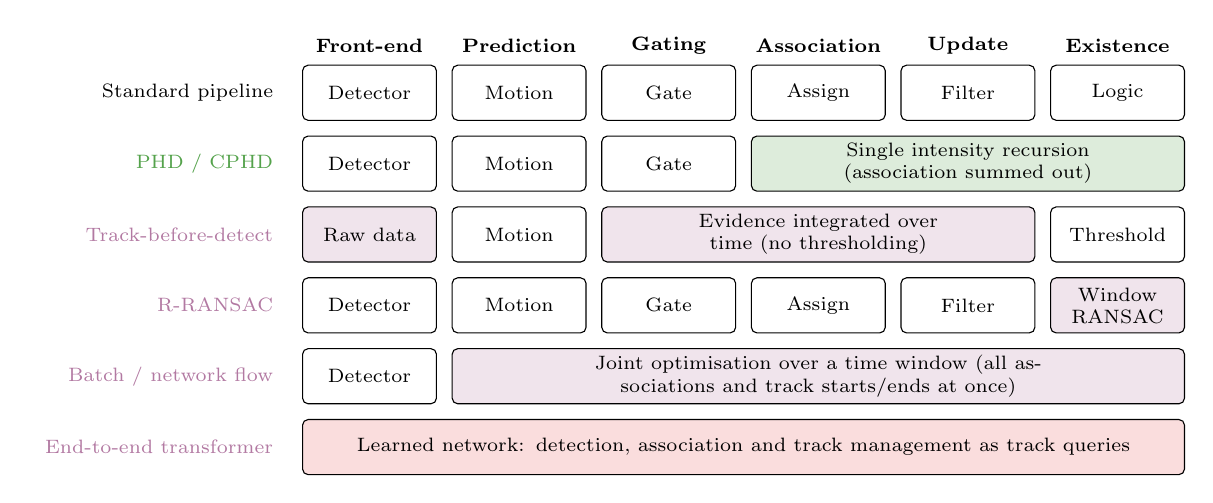
\begin{tikzpicture}[
  blk/.style={draw, rounded corners=2pt, minimum height=0.7cm, font=\scriptsize,
              align=center, fill=white, inner sep=1pt},
  rl/.style={font=\scriptsize, anchor=east, align=right, text width=3.0cm}]
% header
\foreach \i/\t in {0/Front-end, 1/Prediction, 2/Gating, 3/Association, 4/Update, 5/Existence}
  {\node[font=\scriptsize\bfseries] at (\i*1.9, 0.6) {\t};}
% standard
\node[rl] at (-1.1,0) {Standard pipeline};
\foreach \i/\t in {0/Detector,1/Motion,2/Gate,3/Assign,4/Filter,5/Logic}{\mttblk{\i}{\i}{0}{\t}{}}
% PHD
\node[rl] at (-1.1,-0.9) {\textcolor{famIMP}{PHD / CPHD}};
\foreach \i/\t in {0/Detector,1/Motion,2/Gate}{\mttblk{\i}{\i}{-0.9}{\t}{}}
\mttblk{3}{5}{-0.9}{Single intensity recursion (association summed out)}{fill=famIMP!20}
% TBD
\node[rl] at (-1.1,-1.8) {\textcolor{famOUT}{Track-before-detect}};
\mttblk{0}{0}{-1.8}{Raw data}{fill=famOUT!20}
\mttblk{1}{1}{-1.8}{Motion}{}
\mttblk{2}{4}{-1.8}{Evidence integrated over time (no thresholding)}{fill=famOUT!20}
\mttblk{5}{5}{-1.8}{Threshold}{}
% R-RANSAC
\node[rl] at (-1.1,-2.7) {\textcolor{famOUT}{R-RANSAC}};
\foreach \i/\t in {0/Detector,1/Motion,2/Gate,3/Assign,4/Filter}{\mttblk{\i}{\i}{-2.7}{\t}{}}
\mttblk{5}{5}{-2.7}{Window\\RANSAC}{fill=famOUT!20}
% batch / network flow
\node[rl] at (-1.1,-3.6) {\textcolor{famOUT}{Batch / network flow}};
\mttblk{0}{0}{-3.6}{Detector}{}
\mttblk{1}{5}{-3.6}{Joint optimisation over a time window (all associations and track starts/ends at once)}{fill=famOUT!20}
% end-to-end
\node[rl] at (-1.1,-4.5) {\textcolor{famOUT}{End-to-end transformer}};
\mttblk{0}{5}{-4.5}{Learned network: detection, association and track management as track queries}{fill=accLRN!20}
\end{tikzpicture}}
\caption{Methods described by the blocks they fuse (wide boxes) or
  replace (shaded boxes). White boxes are standard blocks.
  \TODO{Check the R-RANSAC strip: it replaces initiation with
  hypothesise-and-test over a sliding window and keeps a filter bank.}}
\label{fig:rewired}
\end{figure}

\paragraph{\textcolor{famOUT}{Track-before-detect.}}
\TODO{Fuses detection, association and update by integrating raw sensor
evidence over time. Gains: low-SNR targets. Costs: heavy computation,
sensor-specific. Dynamic programming, particle and RFS-based (Bernoulli) variants.}
\paragraph{\textcolor{famOUT}{Recursive RANSAC.}}
\TODO{Replaces probabilistic initiation with hypothesise-and-test over a
measurement window; otherwise a bank of filters with heuristic
association. Mostly a different existence block.}
\paragraph{\textcolor{famOUT}{Batch and network-flow methods.}}
\TODO{Solve association over a whole window jointly (min-cost flow,
multi-frame assignment). Related to N-scan MHT; offline or with latency.}
\paragraph{\textcolor{famOUT}{End-to-end learned trackers.}}
\TODO{TrackFormer, MOTR: track queries carry identity across frames,
so association and existence are learned jointly. Gains: no hand-tuned
association. Costs: no explicit uncertainty, large training sets,
domain shift. Contrast with Table~\ref{tab:designspace}, where learning
replaces a single block.}

With all methods placed on the same vocabulary, they can be compared
on common criteria.

% =====================================================================
\subsection{Comparing the families}
\label{sec:compare}

Three lenses are used in turn: \emph{what each method assumes},
\emph{when it breaks}, and \emph{what it costs}.

\subsubsection{Lens 1: assumptions and outputs}

\begin{table}[t]
\centering\small
\caption{Assumptions and outputs by method. \TODO{Verify each cell against the cited sources.}}
\label{tab:compare}
\begin{tabularx}{\textwidth}{>{\raggedright\arraybackslash}p{2.0cm} p{2.3cm} c p{2.6cm} X p{2.0cm}}
\toprule
Method & Target count & Identity & Cost & Key requirements & Multi-sensor \\
\midrule
\rowcolor{famSH!15}  GNN, SORT-family & external logic & \cmark & polynomial & separated targets or appearance cues & sequential \\
\rowcolor{famSM!15}  JPDA, JIPDA & logic / existence & \cmark & exponential (approx.\ exist) & moderate clutter & sequential \\
\rowcolor{famSM!15}  PMB, LMB  & estimated & \cmark & moderate & known $\PD$, clutter rate & sequential \\
\rowcolor{famMH!15}  MHT       & hypothesis-level & \cmark & exponential, pruned & pruning parameters & centralised \\
\rowcolor{famMH!15}  PMBM, $\delta$-GLMB & estimated & \cmark & moderate--high & known $\PD$, clutter rate, birth model & centralised \\
\rowcolor{famIMP!15} PHD/CPHD  & estimated & \xmark & low--moderate & Poisson-type models & approximate \\
\rowcolor{famOUT!15} TBD       & implicit & varies & high & raw data & sensor-specific \\
\rowcolor{famOUT!15} End-to-end & learned & \cmark & GPU inference & training data & mostly single \\
\bottomrule
\end{tabularx}
\end{table}

\subsubsection{Lens 2: failure modes}

\begin{table}[t]
\centering\small
\caption{Qualitative robustness on known difficulties.}
\label{tab:stress}
\begin{tabular}{l c c c c c}
\toprule
Method & Crossing & Dense clutter & Close spacing & Low $\PD$ & Birth/death \\
\midrule
GNN                 & \weak   & \weak   & \weak   & \fair   & \weak \\
SORT-family         & \fair   & \weak   & \fair   & \weak   & \fair \\
JPDA, JIPDA         & \fair   & \fair   & \weak   & \fair   & \fair \\
PMB, LMB            & \fair   & \fair   & \fair   & \fair   & \strong \\
MHT                 & \strong & \fair   & \strong & \strong & \fair \\
PMBM, $\delta$-GLMB & \strong & \fair   & \strong & \strong & \strong \\
PHD/CPHD            & \fair   & \fair   & \weak   & \fair   & \strong \\
TBD                 & \fair   & \strong & \fair   & \strong & \fair \\
End-to-end          & \fair   & \weak   & \fair   & \weak   & \fair \\
\bottomrule
\end{tabular}
\end{table}

\subsubsection{Lens 3: cost versus fidelity}

\begin{figure}[t]
\centering
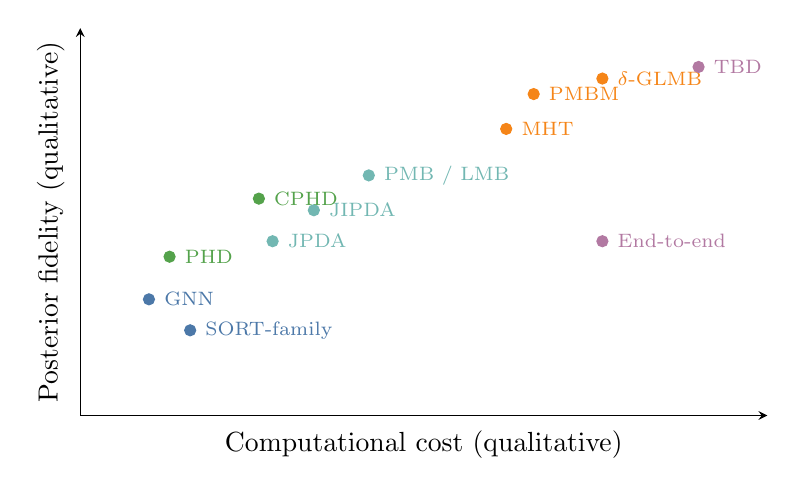
\begin{tikzpicture}
\begin{axis}[width=0.85\textwidth, height=6.5cm, xmin=0, xmax=10, ymin=0, ymax=10,
  xlabel={Computational cost (qualitative)},
  ylabel={Posterior fidelity (qualitative)},
  xtick=\empty, ytick=\empty, axis lines=left,
  nodes near coords, point meta=explicit symbolic,
  every node near coord/.append style={font=\scriptsize, anchor=west, xshift=2pt},
  mark=*]
\addplot[only marks, color=famSH]  coordinates {(1,3) [GNN] (1.6,2.2) [SORT-family]};
\addplot[only marks, color=famSM]  coordinates {(2.8,4.5) [JPDA] (3.4,5.3) [JIPDA] (4.2,6.2) [PMB / LMB]};
\addplot[only marks, color=famMH]  coordinates {(6.2,7.4) [MHT] (6.6,8.3) [PMBM] (7.6,8.7) [$\delta$-GLMB]};
\addplot[only marks, color=famIMP] coordinates {(1.3,4.1) [PHD] (2.6,5.6) [CPHD]};
\addplot[only marks, color=famOUT] coordinates {(9,9) [TBD] (7.6,4.5) [End-to-end]};
\end{axis}
\end{tikzpicture}
\caption{Illustrative cost--fidelity trade-off. Within the
  detection-based families the ordering follows the approximation
  ladder of Fig.~\ref{fig:funnel}. Placement is subjective and for
  orientation only; ``fidelity'' is not well defined for learned
  trackers. \TODO{Replace with measured runtimes/accuracy if you have them.}}
\label{fig:tradeoff}
\end{figure}

Taken together, the three lenses show that no family dominates: the
best choice depends on clutter, target dynamics and available compute.
Because the blocks are independent, the choice is best made block by
block, which the final guide does.

% =====================================================================
\subsection{Design guide and implications for this project}
\label{sec:selection}

\begin{table}[t]
\centering\small
\caption{Design guide, one question per building block.
  \TODO{Adjust after finalising the comparison; optionally condense into a flowchart.}}
\label{tab:selection}
\begin{tabularx}{\textwidth}{>{\raggedright\arraybackslash}p{2.3cm} X X}
\toprule
Block & Question & If yes, lean towards \\
\midrule
Front-end   & Very low SNR, and raw data available? & Track-before-detect \\
Motion model & Manoeuvring targets? Training data for unusual dynamics? & IMM; learned motion model \\
Association cost & Rich appearance cues (e.g.\ EO video)? & Add learned re-ID affinity to the kinematic cost \\
Association decision & Frequent ambiguity (crossings, close spacing, clutter)? & Deferred (MHT, PMBM); otherwise marginal (JIPDA, PMB) or hard (GNN) \\
Representation & Many hypotheses with long shared histories? & Track-oriented (TOMHT, PMBM) \\
Existence   & Frequent births/deaths, long detection gaps, undetected targets? & Probabilistic existence, Poisson undetected model \\
Complexity  & Hard real-time budget? & Gating and clustering always; then capping, small $k$, or marginalisation \\
Multi-sensor & Heterogeneous or distributed sensors? & Centralised if bandwidth allows, else track-to-track fusion \\
\bottomrule
\end{tabularx}
\end{table}

\paragraph{Implications for this project.}
\TODO{Walk through Table~\ref{tab:selection} for your own setting:
heterogeneous sensors, sparse and slow-moving targets, sea-return
clutter, ground truth from AIS. State the resulting recipe (one choice
per block) and which options are ruled out, and why.}

\paragraph{Summary.}
\TODO{Two or three sentences: a tracker is a recipe of interchangeable
blocks; families differ in how many association hypotheses they keep,
which is largely a complexity decision; RFS is a modelling framework
that mainly improves the existence block; and what your project takes
from this.}
